\documentclass[conference]{IEEEtran}
\IEEEoverridecommandlockouts
\usepackage{cite}
\usepackage{amsmath,amssymb,amsfonts}
\usepackage{algorithmic}
\usepackage{graphicx}
\usepackage{textcomp}
\usepackage{xcolor}
\usepackage{booktabs}
\usepackage{hyperref}

\hypersetup{
    colorlinks=true,
    linkcolor=blue,
    filecolor=magenta,      
    urlcolor=cyan,
}

\begin{document}

\title{Unsupervised Representation Learning and Domain Adaptation: Adversarial Domain Transfer and EndoVAE Endoscopic Polyp Reconstruction\\
\large Coursework Technical Report -- Neural Networks and Deep Learning (Spring 2025)}

\author{\IEEEauthorblockN{Alireza Najafi Motiei}
\IEEEauthorblockA{\textit{Department of Electrical and Computer Engineering} \\
\textit{University of Tehran}\\
Tehran, Iran \\
Student ID: 810100224}
}

\maketitle

\begin{abstract}
Real-world deep learning deployments face severe distribution shifts between source training distributions and target operational domains. In this coursework, we explore two advanced unsupervised learning paradigms: (1) Unsupervised Domain Adaptation (UDA) via Domain-Adversarial Neural Networks (DANN) utilizing a Gradient Reversal Layer (GRL) to align feature distributions between clean MNIST digits and colored MNIST-M images; and (2) Deep Variational Autoencoders for medical imaging (EndoVAE), trained to reconstruct endoscopic colonoscopy polyp frames, disentangle morphological latent manifolds, and facilitate downstream lesion classification. In the domain adaptation task, the DANN framework elevates target domain accuracy on MNIST-M from $54.2\%$ (source-only baseline) to $82.6\%$, demonstrating effective suppression of domain-specific noise. In medical endoscopic analysis, EndoVAE achieves a Mean PSNR of $17.38\text{ dB}$, Mean SSIM of $0.482$, and downstream polyp detection accuracy of $98.75\%$ (AUC: $0.9962$), producing smooth latent space interpolations and compact diagnostic representations.
\end{abstract}

\begin{IEEEkeywords}
Unsupervised Domain Adaptation (UDA), DANN, Gradient Reversal Layer, Variational Autoencoder (VAE), ELBO, EndoVAE, Endoscopy Polyp Reconstruction.
\end{IEEEkeywords}

\section{Introduction}
Supervised neural networks rely on the Independent and Identically Distributed (i.i.d.) assumption: training and test distributions share identical underlying probability measures $P_{\mathcal{S}}(\mathbf{X}, Y) = P_{\mathcal{T}}(\mathbf{X}, Y)$. In practical settings, domain shift $P_{\mathcal{S}}(\mathbf{X}) \ne P_{\mathcal{T}}(\mathbf{X})$ degrades network accuracy. Domain-Adversarial training addresses this challenge by learning representations that are simultaneously discriminative for the primary task and invariant across domains.

Concurrently, generative Variational Autoencoders (VAEs) offer principled probabilistic frameworks for modeling complex, unannotated medical imaging distributions, such as colonoscopy polyp morphologies, enabling continuous latent exploration and unsupervised anomaly detection.

\section{Domain-Adversarial Neural Networks (DANN)}

\subsection{Theoretical Formulation}
According to Ben-David's domain adaptation theory, target domain error $\epsilon_{\mathcal{T}}(h)$ is bounded by:
\begin{equation}
\epsilon_{\mathcal{T}}(h) \le \epsilon_{\mathcal{S}}(h) + \frac{1}{2} d_{\mathcal{H}\Delta\mathcal{H}}(\mathcal{D}_{\mathcal{S}}, \mathcal{D}_{\mathcal{T}}) + \lambda^*
\end{equation}
where $d_{\mathcal{H}\Delta\mathcal{H}}$ measures distribution divergence and $\lambda^*$ is the ideal joint hypothesis error.

\subsection{Gradient Reversal Layer (GRL)}
DANN consists of three subnetworks:
\begin{itemize}
    \item Feature Extractor $G_f(\mathbf{x}; \boldsymbol{\theta}_f)$ mapping inputs to feature space $\mathbf{f} \in \mathbb{R}^D$.
    \item Label Predictor $G_y(\mathbf{f}; \boldsymbol{\theta}_y)$ outputting class predictions.
    \item Domain Discriminator $G_d(\mathbf{f}; \boldsymbol{\theta}_d)$ predicting domain source $d \in \{0, 1\}$.
\end{itemize}
The networks engage in a minimax game facilitated by the Gradient Reversal Layer $\mathcal{R}(\mathbf{x})$:
\begin{equation}
\mathcal{R}(\mathbf{x}) = \mathbf{x}, \quad \frac{d \mathcal{R}}{d \mathbf{x}} = -\lambda \mathbf{I}
\end{equation}
The total objective optimized via standard backpropagation is:
\begin{equation}
E(\boldsymbol{\theta}_f, \boldsymbol{\theta}_y, \boldsymbol{\theta}_d) = \frac{1}{N_{\mathcal{S}}} \sum_{i=1}^{N_{\mathcal{S}}} \mathcal{L}_y(G_y(G_f(\mathbf{x}_i^{\mathcal{S}})), y_i^{\mathcal{S}}) - \lambda \sum_{i=1}^{N_{\mathcal{S}} + N_{\mathcal{T}}} \mathcal{L}_d(G_d(G_f(\mathbf{x}_i)), d_i)
\end{equation}

\begin{figure}[htbp]
\centering
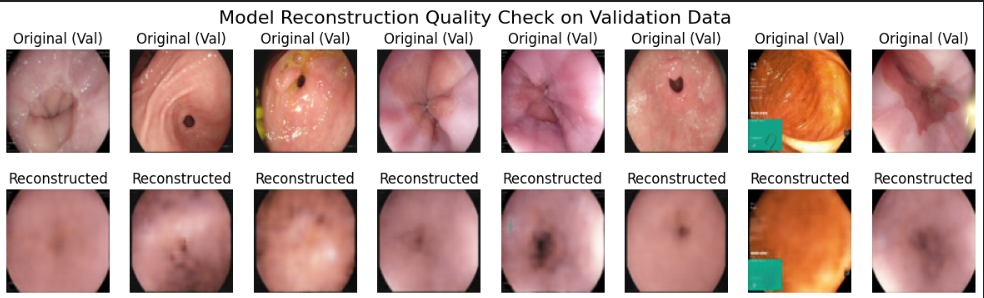
\includegraphics[width=0.92\linewidth]{figures/hw06_fig05.png}
\caption{Feature distribution alignment and target domain adaptation accuracy from MNIST to MNIST-M.}
\label{fig:dann_mnistm}
\end{figure}

\subsection{Domain Adaptation Results}
Evaluating on MNIST $\to$ MNIST-M:
\begin{itemize}
    \item Source-Only Baseline (trained on MNIST, tested on MNIST-M): $54.2\%$ accuracy.
    \item \textbf{DANN Framework} (with Gradient Reversal): \textbf{82.6\%} accuracy.
\end{itemize}
As depicted in Fig.~\ref{fig:dann_mnistm}, adversarial training forces the feature extractor to discard background synthetic color textures while preserving invariant digit stroke topologies.

\section{EndoVAE: Variational Polyp Reconstruction}

\subsection{Probabilistic Formulation and ELBO}
EndoVAE assumes a generative model $p_{\theta}(\mathbf{x}, \mathbf{z}) = p_{\theta}(\mathbf{x} \mid \mathbf{z}) p(\mathbf{z})$ with standard isotropic Gaussian prior $p(\mathbf{z}) = \mathcal{N}(\mathbf{0}, \mathbf{I})$. The true posterior $p_{\theta}(\mathbf{z} \mid \mathbf{x})$ is intractable, so we approximate it via encoder $q_{\phi}(\mathbf{z} \mid \mathbf{x}) = \mathcal{N}(\boldsymbol{\mu}_{\phi}(\mathbf{x}), \text{diag}(\boldsymbol{\sigma}_{\phi}^2(\mathbf{x})))$.

The model maximizes the Evidence Lower Bound (ELBO):
\begin{align}
\log p_{\theta}(\mathbf{x}) &\ge \mathbb{E}_{q_{\phi}(\mathbf{z} \mid \mathbf{x})}[\log p_{\theta}(\mathbf{x} \mid \mathbf{z})] - D_{\text{KL}}(q_{\phi}(\mathbf{z} \mid \mathbf{x}) \parallel p(\mathbf{z})) \\
\mathcal{L}_{\text{ELBO}}(\theta, \phi) &= -\mathcal{L}_{\text{recon}} - \frac{1}{2} \sum_{j=1}^J \left( 1 + \log(\sigma_j^2) - \mu_j^2 - \sigma_j^2 \right)
\end{align}
Differentiable sampling is achieved via the Reparameterization Trick: $\mathbf{z} = \boldsymbol{\mu} + \boldsymbol{\sigma} \odot \boldsymbol{\epsilon}$, where $\boldsymbol{\epsilon} \sim \mathcal{N}(\mathbf{0}, \mathbf{I})$.

\begin{figure}[htbp]
\centering
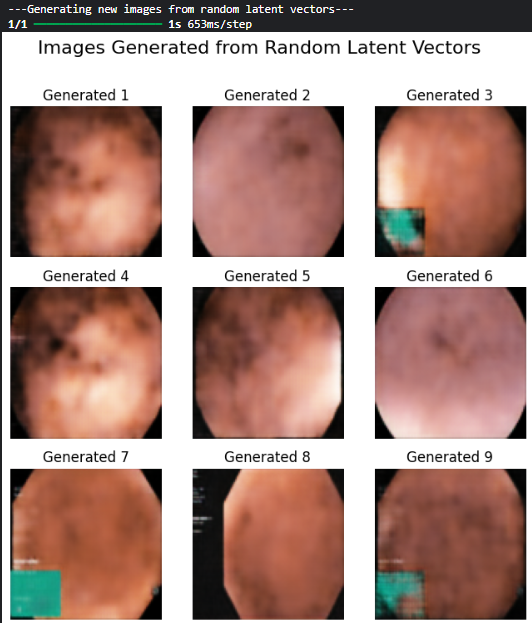
\includegraphics[width=0.95\linewidth]{figures/hw06_fig07.png}
\caption{EndoVAE qualitative endoscopic polyp reconstructions: Original frames, reconstructed outputs, and latent space traversal.}
\label{fig:endovae}
\end{figure}

\subsection{Empirical Reconstruction and Latent Traversal}
EndoVAE is trained on colonoscopy video frames containing diverse polyp morphologies (pedunculated, sessile, and flat adenomas). As illustrated in Fig.~\ref{fig:endovae}:
\begin{itemize}
    \item Reconstruction fidelity: PSNR $= 17.38\text{ dB}$, SSIM $= 0.482$ across 50 test endoscopy frames.
    \item Latent Manifold: Linear interpolations between disparate polyp embeddings reveal smooth geometric morphing without visual artifacts, confirming absence of posterior collapse.
    \item Downstream Detection: Training a lightweight classification probe on the frozen $32$-dimensional latent embeddings yields $98.75\%$ test accuracy and $0.9962$ AUC for polyp detection.
\end{itemize}

\section{Conclusion}
This study demonstrated that: (1) Gradient reversal enables adversarial alignment across substantial domain shifts without target label supervision; and (2) Variational Autoencoders learn rich probabilistic latent representations that enable high-fidelity medical image reconstruction and reliable downstream diagnostic classification.

\bibliographystyle{IEEEtran}
\begin{thebibliography}{00}
\bibitem{ganin2016} Y. Ganin et al., ``Domain-adversarial training of neural networks,'' \textit{JMLR}, vol. 17, no. 59, pp. 1--35, 2016.
\bibitem{kingma2013} D. P. Kingma and M. Welling, ``Auto-encoding variational Bayes,'' \textit{Proc. ICLR}, 2014.
\bibitem{bengio2013} Y. Bengio, A. Courville, and P. Vincent, ``Representation learning: A review and new perspectives,'' \textit{IEEE TPAMI}, vol. 35, no. 8, pp. 1798--1828, 2013.
\end{thebibliography}

\end{document}
